\chapter{Fussballszenario} \label{kap:Fussballszenario} %TODO: Besseren Kapiteltitel

\section{Szenario Koordination} %TODO: Hendrik

\subsection{Kommunikation per RSB und Spread} %TODO: Hendrik

\subsection{Finite-State-Machine} %TODO: Hendrik

\begin{figure}[H]
	\begin{center}
		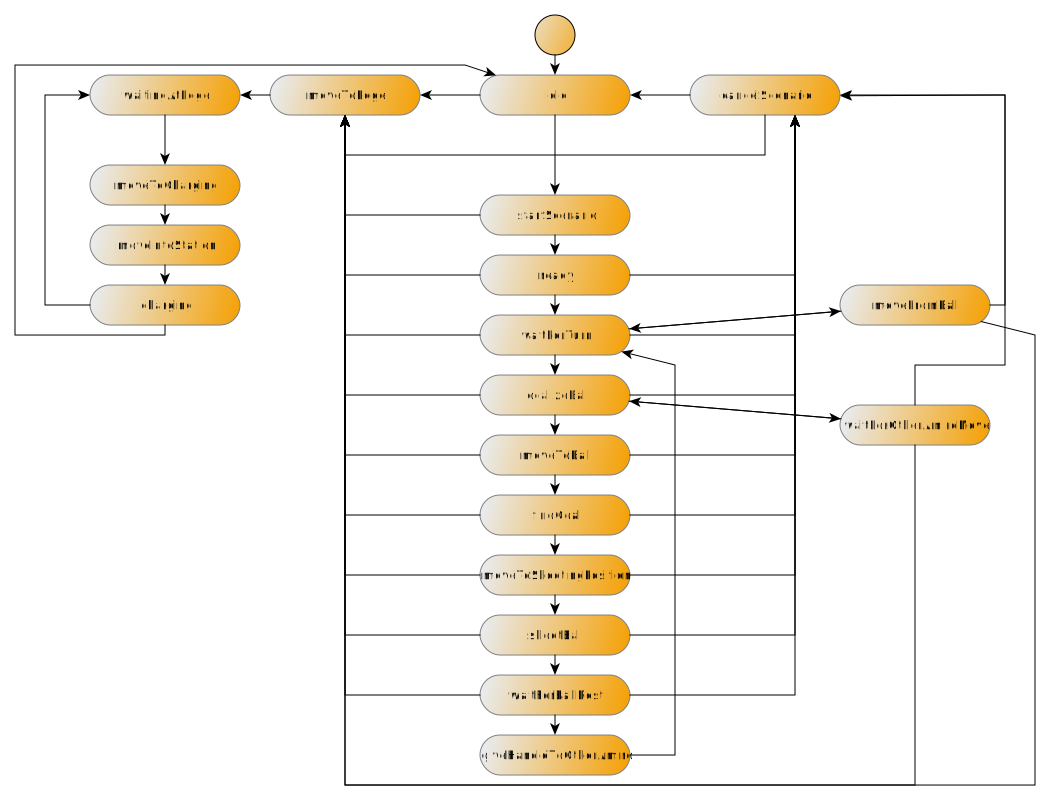
\includegraphics[scale=.55]{Final_FSM_AMiRo.pdf} 	
		\caption{Finite-State-Machine}
		\label{fig:fsm-amiro}
	\end{center}
\end{figure}

\section{Realisierung der einzelnen Spielelemente} %TODO: Besseren Sectiontitel

\subsection{Lokalisation des Balls} %TODO: Julian E.

\subsection{Anfahren des Balls} %TODO: Julian E.

\subsection{Lokalisation des gegnerischen Tores} %TODO: Timo M.

\subsection{Schussposition anfahren} %TODO: Timo M.

\subsection{Schießen} %TODO: Timo M.

\subsection{Beiseite Fahren} %TODO: Julian E. (Besseren Titel suchen^^)

\section{Spieltracking} %TODO: Julian D.

\subsection{Spielfeldbestimmung mit dem AR Toolkit} %TODO: Julian D.

\subsection{Extraktion wichtiger Spielelemente mit Bildverarbeitungsmethoden} %TODO: Julian D.

\subsection{Benutzerinteraktion mit AR Markern} %TODO: Julian D.

\subsection{Spielkoordination} %TODO: Julian D.

\subsection{Grafische Darstellung der Spielstatus} %TODO: Julian D.